\documentclass[t]{beamer}
\usetheme{Warsaw}
\usepackage{array}
\usepackage{graphicx}
\usepackage{amssymb,amsmath,mathrsfs,amsfonts}
%\usepackage[colorhighlight,display]{texpower}
%\usepackage{caption}
%\usepackage[all]{xy}
\usepackage{beamerthemesplit}
\mode<presentation>
%\usepackage{pause}
\usepackage{ulem}  % for strikethroughs
\usepackage{cancel} % for strikethroughs in math mode 
\usepackage{tikz}
\usepackage{calc}
\usetikzlibrary{shapes}
\usepackage{hyperref}
\hypersetup{pdfpagemode=FullScreen}
\usepackage{ifthen}
\usepackage{animate}
\usepackage{color}
\usepackage{type1cm}  % used for watermarking
\usepackage{eso-pic}  % used for watermarking


\theoremstyle{plain}
\newtheorem{prop}{Proposition}
\newtheorem{thm}[prop]{Theorem}
\newtheorem{lem}[prop]{Lemma}
\newtheorem{cor}[prop]{Corollary}
\theoremstyle{definition}
\newtheorem{dfn}{Definition}
\newtheorem{rem}[prop]{Remark}
\newtheorem{ex}{Example}[section]
%\newtheorem{note}{Note}[section]
\newtheorem{exercise}{Exercise}[section]
\newcommand{\nin}{\noindent}
\newcommand{\ds}{\displaystyle}
\renewcommand{\figurename}{Figure \arabic{figure}}



\renewcommand*\familydefault{\sfdefault} 




%%%%%%%%%%%%%%%%%%%%%%%%%%5
%%%%%%%%%%%%%%%%%%%%%%%%%%%%
%%%% some commands that have different meaning in the article/presentation modes

\newcommand{\vvfill}{\mode<presentation>{\vfill}  \mode<article>{\medskip}}   %vfill in presentation only
\newcommand{\sketchspace}{ 
\mode<article>{ \medskip\noindent{\textbf{Sketch:}} \vspace*{6cm} }
\mode<presentation>{ } 
}
\newcommand{\examplespace}{ 
\mode<article>{ \medskip\noindent{\textbf{Example:}} \vspace{6cm} }
\mode<presentation>{ } 
}
\newcommand{\artsmspace}{\mode<article>{\vspace*{2cm}} }  %small space in article mode
\newcommand{\artlargespace}{\mode<article>{\vspace*{6cm}} }  %large space in article mode

\newcommand{\dx}{\,dx}

\newcommand{\soln}{{\textbf{Solution: }}\,\,\,}
\newcommand{\disp}{\displaystyle}

\newcommand{\makedate}{\vvfill
\begin{picture}(10,10)  
\put(260,-20){\mbox{\tiny{\today}}}
\end{picture}
}

\newcommand{\pd}[2]{\dfrac{\partial#1}{\partial#2}}
\newcommand{\pD}[2]{\dfrac{\partial^2#1}{\partial#2^2}}
\newcommand{\pdd}[3]{\dfrac{\partial^2#1}{\partial#2 \partial#3}}


\normalem %stops the ulem package making all the emphs into underlines...
 
 
 
 \newcommand{\refandrev}[2]{
 \begin{small}
  \hspace{6cm}
  \begin{minipage}[r]{8cm}
  Stewart,    Chapter #1   \\
  Review:  \parbox[t]{6cm}{#2}
\end{minipage}
\end{small}
}



\newcounter{heading}
\setcounter{section}{1}
\setcounter{heading}{0}

\newcommand{\makeheading}[1]{\medskip\begin{large}\noindent\textbf{{#1}}\end{large}\smallskip}

%\newenvironment{head}[1]{\medskip\stepcounter{heading}\noindent\textbf{\hspace{0.2cm}{#1}.}}{}
\newcommand{\newhead}[1]{\medskip\stepcounter{heading}\noindent\textbf{\hspace{0.2cm}{#1}.}}


\newcommand{\pf}[1]{\noindent\textit{Proof.}\vspace*{#1 cm}}
\newcommand{\sol}[1]{\noindent\textit{Solution.}\vspace*{#1 cm}}
\newcommand{\further}[1]{\begin{small}\noindent\textit{Further reading: #1}\end{small}}
\newcommand{\exr}[1]{\begin{footnotesize}\noindent\textit{\textbf{Exercises:} Stewart #1}\end{footnotesize}}


% Sets of numbers
\newcommand{\C}{\mathbb{C}}
\newcommand{\RR}{\mathbb{R}}
\newcommand{\Z}{\mathbb{Z}}
\newcommand{\N}{\mathbb{N}}
\newcommand{\Q}{\mathbb{Q}}

% Partitions
\newcommand{\PP}{\mathcal{P}}

% Limits
\newcommand{\limm}[1]{\displaystyle \lim_{x\to #1}}

% Backslash
\newcommand{\bs}{\backslash}

% functions
\newcommand{\cosec}{\mathrm{cosec}}
\newcommand{\cosech}{\mathrm{cosech}}
\newcommand{\sech}{\mathrm{sech}}
\newcommand{\Li}{\mathrm{Li}}
\newcommand{\si}{\mathrm{Si}}
\newcommand{\erf}{\mathrm{erf}}

% Domain and Range
\newcommand{\Dom}{\mathrm{Dom}}
\newcommand{\Codom}{\mathrm{Codom}}
\newcommand{\Range}{\mathrm{Ran}}



\title{Week 9:  The natural logarithm and exponential functions}
\date{October 2 -- October 5, 2012}

\begin{document}

\frame{\titlepage}

\setcounter{tocdepth}{2}
\frame{\tableofcontents

\begin{flushright}
\hyperlink{wed}{\beamergotobutton{Lecture 17}}\\

\hyperlink{thurs}{\beamergotobutton{Lecture 18}}
\end{flushright} 
}

\AtBeginSection[]
{
\begin{frame}<beamer> 
\tableofcontents[currentsection]  % show TOC and highlight current section
\end{frame}
}

\section{The natural logarithm \& exponential}
\subsection{The natural logarithm}

\begin{frame}
\frametitle{Recall from last class}
\uncover<+->{\begin{dfn} The function $\ln$ with domain $(0,\infty)$ is defined by the formula
\[\ln(x)=\int_1^x\frac{1}{t}\,dt.\]\end{dfn}}
\uncover<+->{\noindent By interpreting $\ln$ as the area under a curve, we can see that:}
\begin{itemize}[<+->]
\item $\ln x>0$ if $x>1$ and $\ln1=0$,
\item $\ln x<0$ if $0<x<1$.
\end{itemize}
\uncover<+->{\noindent We have the following (familiar) properties of the logarithm:}
\begin{enumerate}[<+->]
\item[(i)] $\ln(xy)=\ln(x)+\ln(y)$ for all positive real numbers $x$ and $y$.
\item[(ii)] $\ds \ln\big(\tfrac{x}{y}\big)=\ln(x)-\ln(y)$ for all positive real numbers $x$ and $y$.
\item[(iii)] $\ln(x^r)=r\ln(x)$ whenever $r$ is a rational number and $x$ is a positive real number.
\end{enumerate}
\end{frame}

\begin{frame}
\uncover<+->{\newhead{Graphing the natural logarithm} The natural logarithm has the following limits:}
\begin{enumerate}[<+->]
\item[(a)] $\limm{\infty} \ln x = \infty.$
\item[(b)] $\limm{0^{+}} \ln x = -\infty.$
\end{enumerate}
\uncover<+->{Also, if $y  = \ln x$ and $x>0$, 
\[ \frac{dy}{dx} = \frac{1}{x} > 0 \qquad \text{and} \qquad \frac{d^{2}y}{dx^{2}} = -\frac{1}{x^{2}} < 0.\]}
\uncover<+->{Hence $\ln x$ is increasing and concave downward.  Also, $\ln 1 = 0$ and $\ln x$ is continuous, so the graph looks like this:}
\begin{center}
\uncover<+->{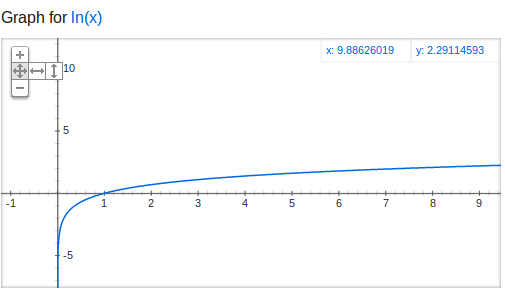
\includegraphics[scale=.3]{Graphofln(x).png}}
\end{center}


\end{frame}

\begin{frame}
\newhead{\textbf{Important definition}}  By the intermediate value theorem, there is a number where $\ln x$ equals $1$.  We denote this number by $e$ (for ``Euler").  It is (in my opinion) perhaps the most important number in mathematics.  It is irrational, and \textbf{approximately} equal to  $2.718$.\pause

\vspace*{.4cm}

\newhead{Example} Differentiate the function given by $y = \ln(\sin x)$.
\end{frame}

\begin{frame}
\newhead{Remarks}
\begin{itemize}[<+->]
\item In general, $\frac{d}{dx}\ln (g(x)) = \frac{g'(x)}{g(x)}$.  
\item Note that when we consider function like $\ln(g(x))$, we are assuming that this composite function is defined on some interval $I$ such that the range of $g$, when restricted to $I$, lies in the domain of definition of $\ln$.  \emph{The book does not emphasize this, which can be somewhat confusing.}
\end{itemize}

\uncover<+->{\vspace*{1cm}
\newhead{Example} Suppose $f$ is defined by $f(x) = \ln |x|$.  What is $f'(x)$?}

\end{frame}

\begin{frame}
\noindent We record this formula:
\[ \frac{d}{dx} \ln |x| = \frac{1}{x}.\]
Hence, we obtain the formula
\[ \int \frac{1}{x} \, dx = \ln|x| + C.\]\pause

\vspace*{.5cm}

\noindent More generally, we can use the chain rule to derive:
\[\frac{d}{dx}\ln|f(x)|=\frac{f'(x)}{f(x)}\]\pause
hence,
\[\int \frac{f'(x)}{f(x)}\, dx = \ln|f(x)| + C\]
provided that $f$ is differentiable and restricted to an interval $I$ where it is nonzero.
\end{frame}

\begin{frame}
\newhead{Example} Evaluate $\int \frac{x}{x^{2}+1} \,dx$\pause

\vspace*{1cm}

\newhead{Example} Evaluate  $\ds\int\tan x\,dx$. \pause (This example appears in the book on Page 259.  Note that although the book doesn't specify the domain of $x$, it is assumed to be an interval $I$ where $\tan x$ is defined.)
\end{frame}

\begin{frame}
\frametitle{Logarithmic differentiation}

\noindent By taking the logarithm, any problem involving powers, products and quotients can be transformed into a problem involving products, sums and differences. This is a powerful strategy if it is easy to manipulate the resulting logarithms, as is the case with differentiation.\pause

\vspace*{1cm}

\newhead{Example}
Find $\ds\frac{dy}{dx}$ if $\ds y=\left(\frac{(3x^2+4)(x+2)}{x^3+5x}\right)^{3/5}$ and $x>0$.

\end{frame}

\subsection{The exponential function}

\begin{frame}
\makeheading{The exponential function}

\noindent Since $\frac{d}{dx}\ln x=\frac{1}{x} > 0$ on $(0,\infty)$, $\ln x$ is an increasing differentiable function, hence it has a differentiable inverse, which we denote by $\exp$.  The domain of $\exp$ is $\mathbb{R}$ and the range of $\exp$ is $(0, \infty)$.\pause


\newhead{The graph of $\exp$} 

\noindent Reflect the graph of $\ln$ about the line $y=x$.\pause

\vspace*{.3cm}

\noindent Notice that 
\begin{itemize}[<+->]
\item $\exp(0) = 1$ since $\ln(1) = 0$.
\item $\exp(1) = e$ since $\ln(e) = 1$.
\item $\exp(\ln(x)) = x$ and $\ln(\exp(x)) = x$.
\end{itemize}
\end{frame}

\begin{frame}
\noindent Recall that if $r$ is a \emph{rational} number, then 
\[ \ln(e^{r}) = r\ln(e) = r\]  

\pause

\noindent Since $\ln$ and $\exp$ are inverses, this means that $\exp(r) = e^{r}$.\pause

\medskip

\noindent Now $e^{x}$ is currently defined only when $x$ is \emph{rational}, and by the above, it agrees with $\exp(x)$.  But $\exp(x)$ is defined for all \textbf{real} $x$, not just all rational $x$. \pause So we \emph{define} $e^{x} = \exp(x)$ for all irrational $x$ also!  Now $e^{x}$ makes sense for all $x \in \mathbb{R}$.  Therefore,
\[ e^{x} = y \qquad \text{and} \qquad \ln y = x.\]\pause

\noindent Also, the cancellation equations $\exp(\ln(x)) = x$ and $\ln(\exp(x)) = x$ become
\[ e^{\ln x} = x \qquad \text{and} \qquad \ln(e^{x}) = x.\]
The first cancellation formula requires $x>0$, but the second holds for all $x$.
\end{frame}

\begin{frame}
\newhead{Examples}
Simplify the following
\begin{enumerate}[<+->]
\item[(a)] $\ln\sqrt{e}$

\vspace*{.1cm}

\item[(b)] $e^{3\ln 2}$

\vspace*{.1cm}

\item[(c)] $e^{x + \ln x}$
\end{enumerate}
\vspace*{.1cm}
\uncover<+->{\noindent Solve each equation for $x$:}
\begin{enumerate}[<+->]
\item[(d)] $2^{x-5} = 3$

\vspace*{.2cm}

\item[(e)] $\ln x + \ln(x-1) = 1$
\end{enumerate}

\end{frame}

\begin{frame}
\noindent Here are some properties of the exponential function which we can see from the graph:
\vspace*{.1cm}
\begin{itemize}[<+->]
\item $e^{x} > 0$ for all $x$.
\item $\limm{-\infty}e^{x} = 0$.
\item $\limm{\infty}e^{x} = \infty$.
\end{itemize}

\vspace*{.1cm}

\uncover<+->{\noindent We also have the expected nice properties of the exponential function.  If $x, y$ are real and $r$ is rational, then}
\begin{enumerate}[<+->]
\item $e^{x+y} = e^{x}e^{y}$
\item $e^{x-y} = \frac{e^{x}}{e^{y}}$
\item $(e^{x})^{r} = e^{rx}.$
\end{enumerate}
\end{frame}



\end{document}